\documentclass[conference]{IEEEtran}
\IEEEoverridecommandlockouts
% The preceding line is only needed to identify funding in the first footnote. If that is unneeded, please comment it out.
\usepackage{cite}
\usepackage{amsmath,amssymb,amsfonts}
\usepackage{algorithmic}
\usepackage{graphicx}
\usepackage{textcomp}
\usepackage{xcolor}
\usepackage{listings}

\definecolor{dkgreen}{rgb}{0,0.6,0}
\definecolor{gray}{rgb}{0.5,0.5,0.5}
\definecolor{mauve}{rgb}{0.58,0,0.82}

\lstset{frame=tb,
  language=java,
  aboveskip=3mm,
  belowskip=3mm,
  showstringspaces=false,
  columns=flexible,
  basicstyle={\small\ttfamily},
  numbers=none,
  numberstyle=\tiny\color{gray},
  keywordstyle=\color{blue},
  commentstyle=\color{dkgreen},
  stringstyle=\color{mauve},
  breaklines=true,
  breakatwhitespace=true,
  tabsize=3
}
\lstdefinestyle{mystyle}{
  numberstyle=\tiny\color{codegray},
  basicstyle=\footnotesize,
  breakatwhitespace=false,         
  breaklines=true,                 
  keepspaces=true,                 
  numbers=none,                    
  showspaces=false,                
  showstringspaces=false,
  showtabs=false,                  
  tabsize=2
}


\lstset{style= mystyle}

\def\BibTeX{{\rm B\kern-.05em{\sc i\kern-.025em b}\kern-.08em
    T\kern-.1667em\lower.7ex\hbox{E}\kern-.125emX}}
\begin{document}

\title{2D Polygon Triangulation}

\author{\IEEEauthorblockN{Ignacio Barquero Garcia$^{1}$, Jose Pablo Feng$^{2}$, Paul Villafuerte Beita$^{3}$}
\IEEEauthorblockA{\textit{Instituto Tecnologico de Costa Rica (ITCR)} \\
\textit
Cartago, Costa Rica \\
ibarqueroga@gmail.com, joseph.feng1@gmail.com,paulvillabeita@gmail.com}
}

\maketitle
\section{Abstract}
Abstract here
\section{Introduction}
Game figures and models that are visible in a computer screen and pretty much any other polygon can be deconstructed into triangles. This process is called \textbf{triangulation}. In the following project, the chosen triangulation approach is the Ear Clipping path in order to "deconstruct" simple polygons.. Only 2D and \textbf{non-simple polygons} (meaning one or more vertex are shared among various triangles or edges between two vertices that are intersected by other edge) are tested in this project. Additionally, no additional vertices will be inserted.
$$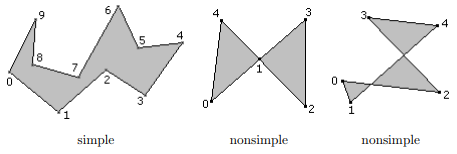
\includegraphics[scale=0.8]{nonsimpleExample}$$
\section{Related Work}
A similar project related to ours is "Fast Poplygon Triangulation Based on Seidel's Algorithm" conducted by Atul Narkhede and Dinesh Manocha. As the title of the project suggests, the use of the Seidel's Algorithm was key. It uses the structure of undirected, unweighted, and connected graphs. It solves the problem in $O(n*logn)$ with polygons that do not have holes and using a query structure to locate a point in logarithmic time.

\section{Computer Graphics}
The term "computer graphics" refers to anything involved in the creation or manipulation
of images on computer, including animated images.\cite{ComputerGraphics}. This is a very broad field, because it includes, for example, 2D and 3D images, such as animated images. For this paper we will be focused only on planar objects. Planar objects, sometimes called 2D shapes, are created on a single plane (usually the xy-plane). Focusing on planar objects, 2D primitives like lines, circles, etc. may be used to create more complex shapes.\cite{2DGraphics}. These graphics are often preferred over 3D because they give more control over the images, and it is very easy to escalate or rotate them.\\
Computer graphics first appeared in the 50's, and one of the firsts and more popular computer game was Spacewar!, developed at MIT by Steve Russell. It took the team about 200 man-hours to write the first version of Spacewar. Russell wrote Spacewar on a PDP-1, an early DEC (Digital Equipment Corporation) interactive mini computer which used a cathode-ray tube type display and keyboard input.\cite{SpaceWar}. Since then, 2D graphics have been being improved and now there are more and better algorithms and techniques that allow us easily keep developing 2D computer graphics.

\section{Polygon Triangulation}
Computing the triangulation of a polygon is a fundamental algorithm in computational
geometry. It also seems to be the most investigated partitioning method\cite{Triangulation}. \\Polygon Triangulation is the decomposition of a polygon in a surface or plane, into a set of triangles, with the restriction that each triangle side is entirely shared by two adjacent triangles. In computer graphics, polygon triangulation algorithms are widely used for tessellating curved geometries. Triangulation can be applied to both convex and concave polygons. Concave polygons are those that have internal angles greater than 180 degrees, convex polygons are the opposite, internal angles sum 180 or less degrees. The Triangulation Theorem states that:
\begin{itemize}
    \item{Every simple polygon admits a triangulation}
\item{Every triangulation of an n-gon has exactly $n-2$ triangles}
\end{itemize}
$$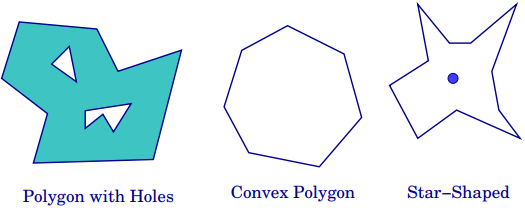
\includegraphics[scale=0.6]{Typeofpolygons}$$
\subsection{Triangulation Approaches}
    \subsubsection{\textbf{Non-Delaunay Algorithms}}
    \begin{itemize}
        \item{Greedy Triangulation}
        \item{Triangulation of Garey et.al}
        \item Ear Clipping / Ear Trimming
        \item{Radial Sweep}
    \end{itemize}
    \subsubsection{\textbf{Delaunay Algorithms}}
    \begin{itemize}
        \item Delaunay triangulation is proposed by B. Delaunay in 1934. Delaunay triangulation maximizes the minimum angles in triangles and avoids skinny triangles.
        \item Delaunay triangulation T of P is a triangulation of P such that the circum-circle of any triangle belonging to T does not contain points of P in its interior.
        \subsubsection{Properties}
        \begin{itemize}
            \item Local empty-circle property
            \item Max-min angle property
            \item Uniqueness
            \item Boundary property
        \end{itemize}
        \subsubsection{Algorithms}
        \begin{itemize}
            \item Incremental Algorithms
            \item Filliping Algorithm
            \item Plane Sweep Algorithm
            \item Divide and Conquer Algorithm
        \end{itemize}
    \end{itemize}
\section{Ear Clipping}
An ear of a polygon is a triangle formed by three consecutive vertices $V_{i0},V_{i1},$ and $V_{i2}$ for which $V_{i1}$ is a convex vertex. The line segment from $V_{i0}$ to $V_{i2}$ lies completely inside the polygon, and no vertices of the polygon are inside the triangle other than its components. The line segment between $V_{i0}$ and $V_{i2}$ is a diagonal of the polygon. The vertex $V_{i1}$ is called the ear tip. A triangle has only one ear and can be any of the triangle's vertices. The Ear Clipping algorithm takes $O(n^2)$.
\section{Experimentation}
For the experimentation process, a background image was set to be used as a guideline and then manually, add vertices in order to enclose the image and create either a convex or concave 2D polygon.
\subsection{Code Analysis}
\begin{lstlisting}
    public void triangulatePolygon() {
      
        long start = System.currentTimeMillis(); //1
        boolean clockwise = isClockwise(points); //n
        int index = 0; //1
        if (points.size() < 3) { //1
            points.clear(); //1
        }else{
            while (points.size() > 2) { //n+1

              Point p1 = points.get((index + 0) % points.size());//1
              Point p2 = points.get((index + 1) % points.size());//1
              Point p3 = points.get((index + 2) % points.size());//1

            Vector v1 = new Vector(p2.x - p1.x, p2.y - p1.y);//1+1
            Vector v2 = new Vector(p3.x - p1.x, p3.y - p1.y);//1+1
                double cross = v1.cross(v2);//1+1
                Polygon triangle = new Polygon(); //1
                triangle.addPoint(p1.x, p1.y); //1
                triangle.addPoint(p2.x, p2.y); //1
                triangle.addPoint(p3.x, p3.y); //1

                if (!clockwise && cross >= 0 && validTriangle(triangle, p1, p2, p3, points)) { //1+n
                    points.remove(p2);//1
                    triangles.add(triangle);//1
                }
                else if (clockwise && cross <= 0 && validTriangle(triangle, p1, p2, p3, points)) { //1+n
                    points.remove(p2);//1
                    triangles.add(triangle);//1
                }
                else {
                    index++;//1
                }
            }
            long end = System.currentTimeMillis();//1
            long time = end-start;//1+1
            long minutes = (time / 1000)  / 60;//1+1
            long seconds = (time / 1000) % 60;//1+1
            long milli = time - (seconds * 1000) - (minutes * 60000);//1
            String report = "Time taken: " + minutes + " min " + seconds + " sec " + milli +" ms" ; //1
            JOptionPane.showMessageDialog(null,report);
        }
    }
\end{lstlisting}
triangulatePolygon Cost =
\newline
$(1)*19 +(2)*5+(n)+((n+1)*(1+n))$
\newline
$19+10+n+(n+n^2+1+n^2)$
\newline
$29+n+(n^2+n+1)$
$30+n+n^2$
$$\therefore O(n^2)$$
\section{Results}
After conducting this part of the experiment, the results showed that the amount of vertices versus time can be different across different polygons based on the contour of the images. This is because there are images that, after enclosing them in a convex hull formed by the vertices, can be simple polygons more than others, that is, that have more edges, bends, curves, etcetera. So, the algorithm needs to check if the new triangle formed by the inclusion of a new vertex is a valid one or not. In synthesis, if a polygon has a lot of vertices, that means that the algorithm will take more time testing each of its vertices; therefore, taking more time to triangulate said polygon. Figure 12 shows the graph corresponding to the Totoro image test, and can give a glimpse of the $n^2$ behaviour even though the line is not very steep.
\begin{figure}
    \centering
    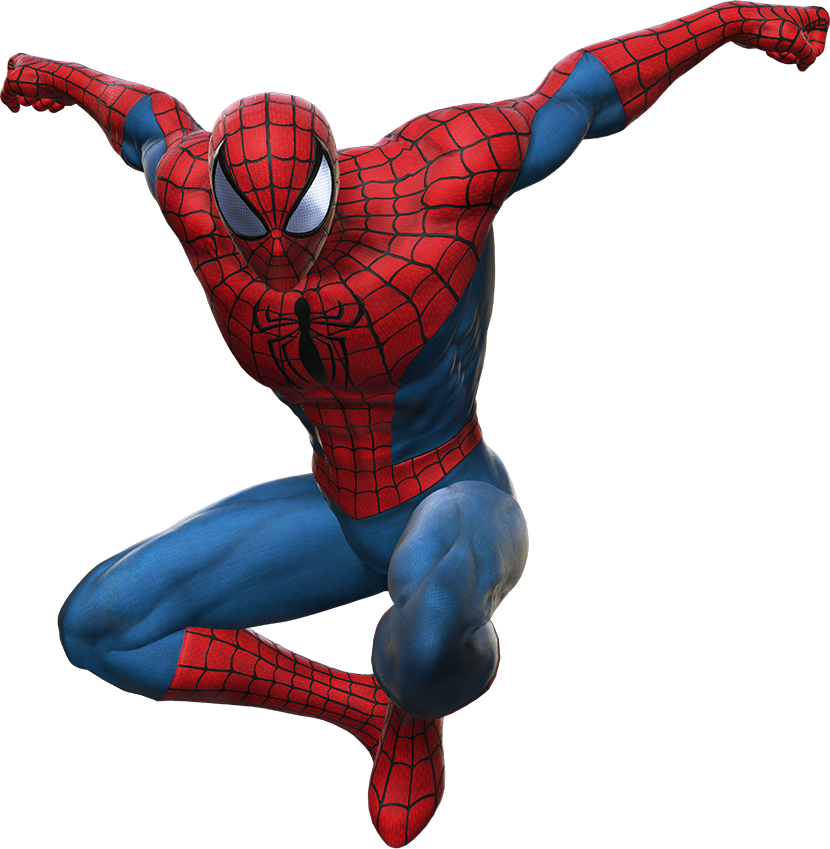
\includegraphics[scale=0.15]{spiderman.png}
    \caption{Test Image}
    \label{fig:testImage}
    \centering
    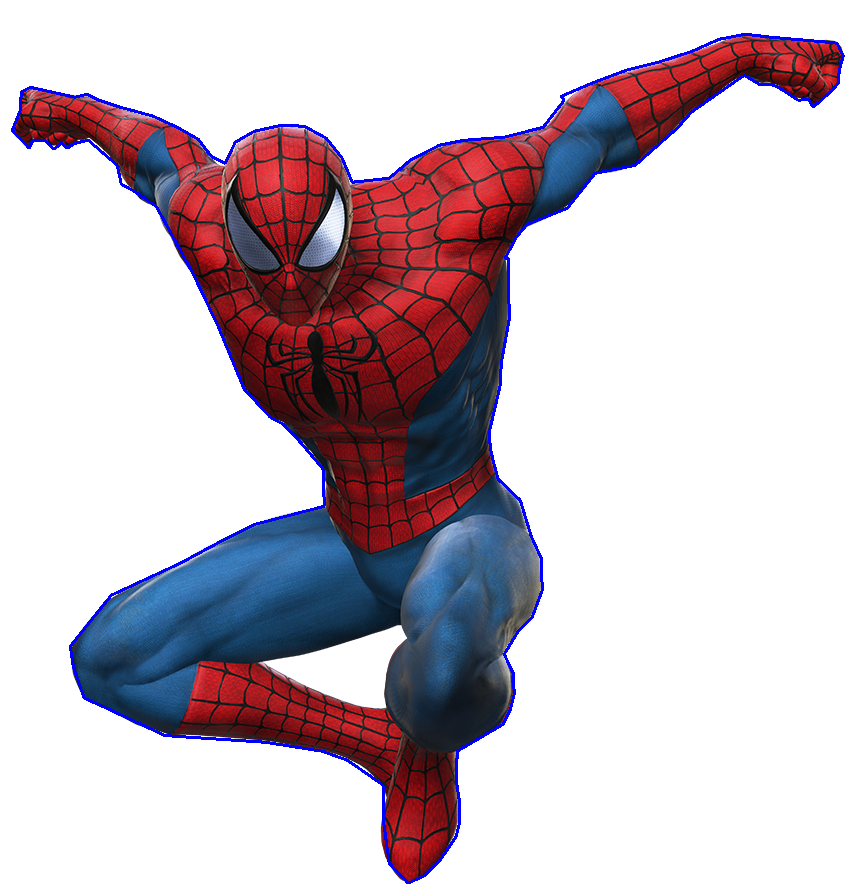
\includegraphics[scale=0.2]{spidermanEnclosed}
    \caption{Test image with 122 vertices}
    \label{fig:test122}
     \centering
    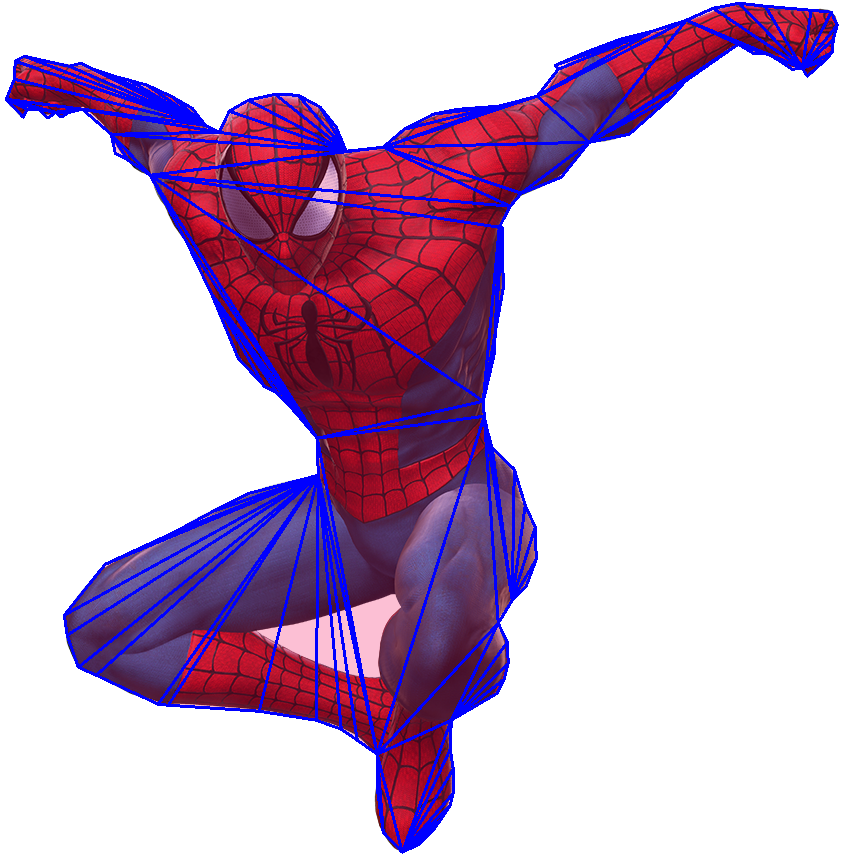
\includegraphics[scale=0.2]{spidermanTriangulated}
    \caption{Fig2 triangulated}
    \label{fig:test122T}
    \centering
    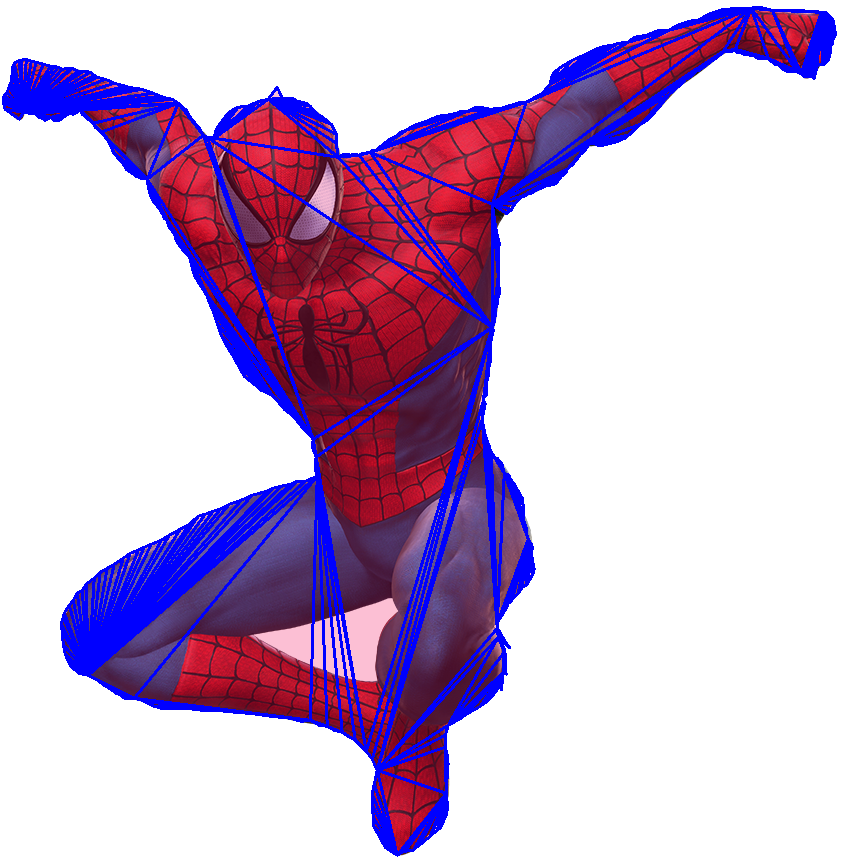
\includegraphics[scale=0.2]{spiderman595Triangulated}
    \caption{Triangulated Spider-Man image with 595 vertices}
    \label{fig:test595}
\end{figure}
\begin{figure}
    \centering
    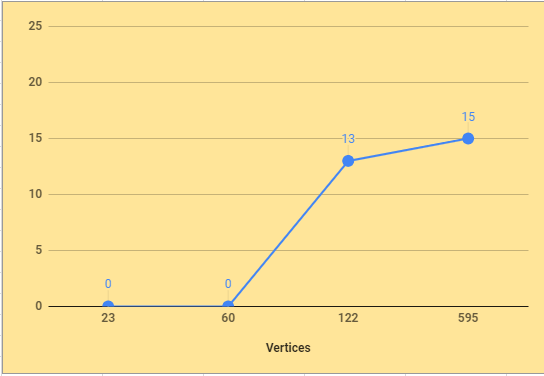
\includegraphics[scale=0.5]{spidermanGraph}
    \caption{Spider-Man Triangulation Results}
    \label{fig:graphspider}
\end{figure}
\begin{figure}
    \centering
    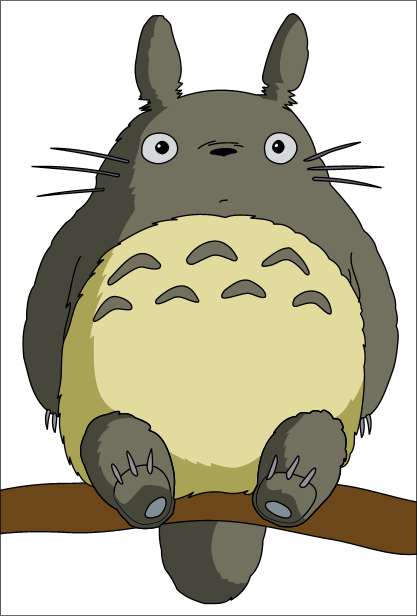
\includegraphics[scale=0.3]{totoro}
    \caption{Test Image 2}
    \label{fig:testImage2}
\end{figure}
\begin{figure}
    \centering
    
\includegraphics[scale =0.3]{totoro1Enclosed}
    \caption{Second test image with 146 vertices}
\end{figure}
\begin{figure}
    \centering
    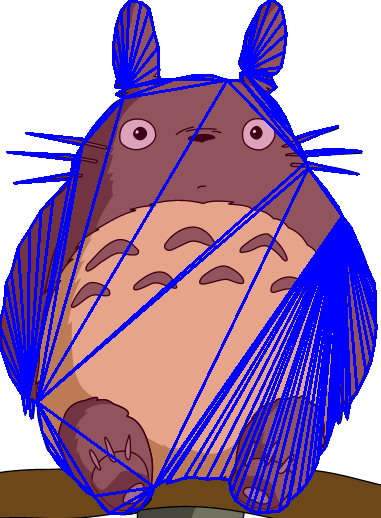
\includegraphics[scale =0.3]{totoro146Triangulated}
    \caption{Second test image with 146 vertices triangulated}
\end{figure}
\begin{figure}
    \centering
    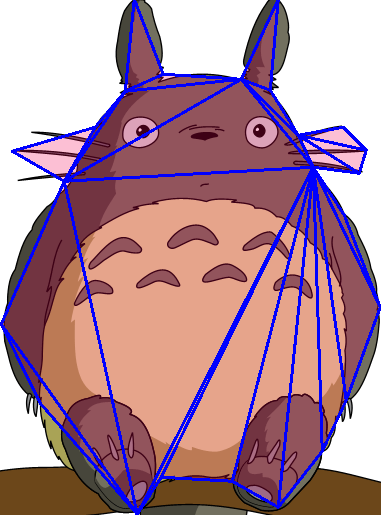
\includegraphics[scale=0.3]{totoro24Triangulated}
    \caption{Second test image with 24 vertices triangulated}
\end{figure}
\begin{figure}
    \centering
    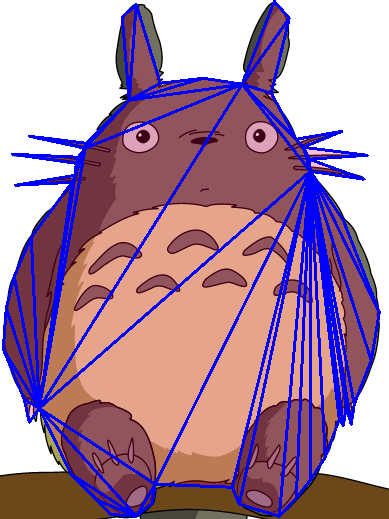
\includegraphics[scale=0.3]{totoro52Triangulated}
    \caption{Second test image with 52 vertices triangulated}
\end{figure}
\begin{figure}
  \centering
    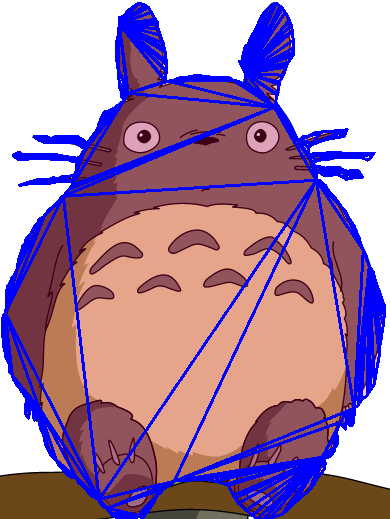
\includegraphics[scale=0.3]{totoro692Triangulated}
    \caption{Second test image with 692 vertices triangulated}
\end{figure}
\begin{figure}
    \centering
    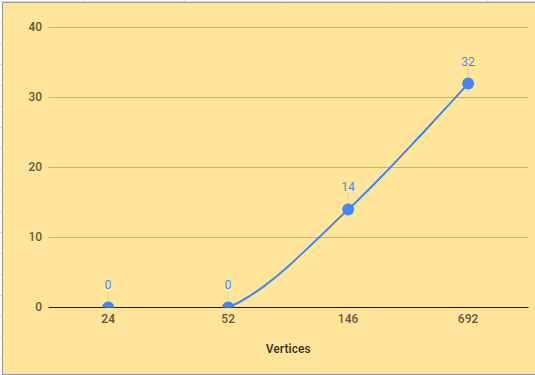
\includegraphics[scale=0.6]{totoroGraph}
    \caption{Totoro Triangulation Results}
    \label{fig:graphtotoro}
\end{figure}

\bibliographystyle{plain}
\bibliography{references}
\end{document}

